\subsection{Package \lstinline{edu.kit.wavelength.client.model}}
\label{pkg:edu.kit.wavelength.client.model}
The \texttt{\pkglnk{model}} package contains the \texttt{\lnk{ExecutionEngine}}
class, which is the primary interface provided by the model to the view for working
with lambda terms. It is initialized with an input string, as well as the reduction
order (see \texttt{\pkglnk{model.reduction}}), output size (see \texttt{\pkglnk{model.output}})
and libraries (see \texttt{\pkglnk{model.library}}) to be used and can then be used to
interactively operate on the lambda term, by stepping forward (that is, $\beta$-reducing
according to the reduction order or reducing a provided redex in the current term)
and backward (reverting to the previous term that was displayed).

The \texttt{\lnk{ExecutionEngine}} is fully synchronous and does not have a notion
of "fully" reducing a term.

\begin{figure}[H]
	\centering
	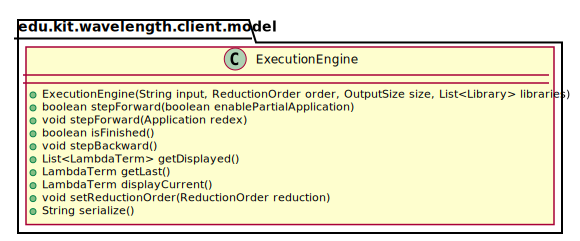
\includegraphics[width=\textwidth]{packageDiagrams/modelPackage}
\end{figure}


\subsubsection{Class \texttt{ExecutionEngine}}
\label{type:edu.kit.wavelength.client.model.ExecutionEngine}
An execution engine manages the reduction of a lambda term.
 It keeps the history of terms and which of these terms were
 displayed and is able to reduce the current term according
 to a reduction order or reduce a specific redex in the current
 term. It also keeps track of which terms should be displayed and
 is able to revert to the previous displayed term.

Constructors:
\begin{itemize}
\item \texttt{ExecutionEngine(String input, \hyperref[type:edu.kit.wavelength.client.model.reduction.ReductionOrder]{ReductionOrder} order, \hyperref[type:edu.kit.wavelength.client.model.output.OutputSize]{OutputSize} size, List<\hyperref[type:edu.kit.wavelength.client.model.library.Library]{Library}> libraries)}

Creates a new execution engine.

\texttt{input}: The textual representation of a lambda term to be handled

\texttt{order}: The reduction order to be used by default

\texttt{size}: The output size to be used

\texttt{libraries}: The libraries to be taken into consideration during parsing

\end{itemize}

Methods:
\begin{itemize}
\item \texttt{boolean stepForward(boolean enablePartialApplication)}

Executes a single reduction of the current lambda term.

\texttt{enablePartialApplication}: Whether partial applications
 and acceleration are enabled

Returns: Whether this step is displayed

\item \texttt{void stepForward(\hyperref[type:edu.kit.wavelength.client.model.term.Application]{Application} redex)}

Executes a single reduction of the supplied redex.

\texttt{redex}: The redex to be evaluated. Must be a redex, otherwise an
 exception is thrown

\item \texttt{boolean isFinished()}

Determines whether the execution is finished according to the current reduction order.

Returns: \texttt{true} if the current reduction order does not provide another redex,
 \texttt{false} otherwise.

\item \texttt{void stepBackward()}

Reverts to the previously output lambda term.

\item \texttt{List<\hyperref[type:edu.kit.wavelength.client.model.term.LambdaTerm]{LambdaTerm}> getDisplayed()}

Returns a list of all lambda terms that have been displayed.

Returns: A list of all lambda terms that have been displayed

\item \texttt{\hyperref[type:edu.kit.wavelength.client.model.term.LambdaTerm]{LambdaTerm} getLast()}

Returns the last lambda term that has been displayed.

Returns: The last lambda term that has been displayed

\item \texttt{\hyperref[type:edu.kit.wavelength.client.model.term.LambdaTerm]{LambdaTerm} displayCurrent()}

Displays the currently reduced term, adding it to the list of displayed terms.

Returns: the current term

\item \texttt{void setReductionOrder(\hyperref[type:edu.kit.wavelength.client.model.reduction.ReductionOrder]{ReductionOrder} reduction)}

Changes the active reduction order to the entered one.

\texttt{reduction}: The new reduction order

\item \texttt{String serialize()}

Serializes the ExecutionEngine by serializing its current OutputSize, ReductionOrder and the terms it holds.

Returns: The ExecutionEngine's serialized String representation

\end{itemize}

\subsection{Package \lstinline{edu.kit.wavelength.client.model.library}}
\label{pkg:edu.kit.wavelength.client.model.library}
The \texttt{\pkglnk{model.library}} contains classes representing the different libraries provided by the application.
Each library consists of a collection of commonly needed \texttt{\hyperref[type:edu.kit.wavelength.client.model.term.LambdaTerm]{LambdaTerm}}s and corresponding names used to reference them.
After enabling a library  these names can be used in place of the longer and more difficult to work with terms.

The \texttt{\lnk{Boolean}} library contains the terms representing the boolean values "true" and "false".

The \texttt{\lnk{TuplesAndLists}} library contains the terms implementing tuples and lists and the functions needed to work with them.

The \texttt{\lnk{NaturalNumbers}} library contains the church encodings of the natural numbers and terms implementing basic arithmic functions.

The \texttt{\lnk{YCombinator}} library contains the Y combinator making recursive function calls possible.

All libraries implement the \texttt{\lnk{Library}} interface allowing the application to be expanded with more libraries provided they too implement this interface.

The library classes are used by the \texttt{\hyperref[type:edu.kit.wavelength.client.model.term.parsing.Parser]{Parser}} 
to access the terms belonging to names in the input String. 
After it has been successfully parsed each used library term is represented by a
\texttt{\hyperref[type:edu.kit.wavelength.client.model.term.NamedTerm]{NamedTerm}} 
in the \texttt{\hyperref[type:edu.kit.wavelength.client.model.term.LambdaTerm]{LambdaTerm}} object structure.

\begin{figure}[H]
	\centering
	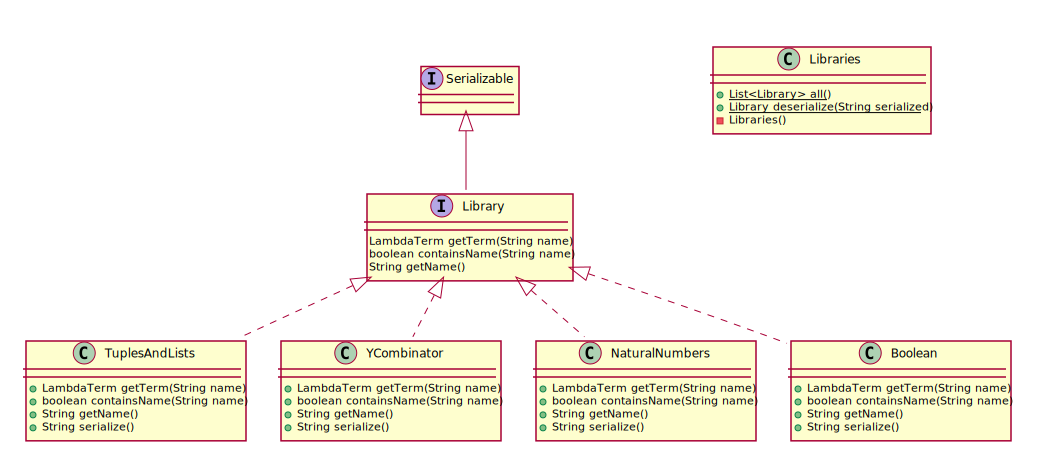
\includegraphics[width=\textwidth]{packageDiagrams/libraryPackage}
\end{figure}

\subsubsection{Class \texttt{YCombinator}}
\label{type:edu.kit.wavelength.client.model.library.YCombinator}
Implements: \texttt{\hyperref[type:edu.kit.wavelength.client.model.library.Library]{Library}}

A library containing the Y combinator.

\subsubsection{Class \texttt{TuplesAndLists}}
\label{type:edu.kit.wavelength.client.model.library.TuplesAndLists}
Implements: \texttt{\hyperref[type:edu.kit.wavelength.client.model.library.Library]{Library}}

A library providing operations for working with
 tuples and lists.

\subsubsection{Class \texttt{NaturalNumbers}}
\label{type:edu.kit.wavelength.client.model.library.NaturalNumbers}
Implements: \texttt{\hyperref[type:edu.kit.wavelength.client.model.library.Library]{Library}}

A library matching integer literals to church numerals
 and providing functions for basic arithmetic operations.

\subsubsection{Interface \texttt{Library}}
\label{type:edu.kit.wavelength.client.model.library.Library}
Extends: \texttt{\hyperref[type:edu.kit.wavelength.client.model.serialization.Serializable]{Serializable}}

This interface is used to interact with the different libraries provided by the application.
 Each library contains a set of lambda terms and their assigned names.
 These names can be used in place of terms to both shorten terms and make them easier to understand.

Methods:
\begin{itemize}
\item \texttt{\hyperref[type:edu.kit.wavelength.client.model.term.LambdaTerm]{LambdaTerm} getTerm(String name)}

Returns the LambdaTerm with the specified name.

\texttt{name}: The name assigned to the desired term

Returns: The term with the entered name, null on error

\item \texttt{boolean containsName(String name)}

Determines whether the library contains a term with the specified name.

\texttt{name}: The name to search the library for

Returns: True if the library contains a term with the entered name

\item \texttt{String getName()}

Returns the library's name

Returns: The name of the library

\end{itemize}

\subsubsection{Class \texttt{Libraries}}
\label{type:edu.kit.wavelength.client.model.library.Libraries}
Static class giving access to all libraries known to the model.

Static methods:
\begin{itemize}
\item \texttt{List<\hyperref[type:edu.kit.wavelength.client.model.library.Library]{Library}> all()}

Returns an unmodifiable list of all libraries known to the model.

Returns: An unmodifiable list that contains exactly one instance of every
         library known to the model

\item \texttt{\hyperref[type:edu.kit.wavelength.client.model.library.Library]{Library} deserialize(String serialized)}

Returns the library referred to by the serialized string.

\texttt{serialized}: A string created by calling serialize on a library known to the
            Libraries class

Returns: The library referred to by the serialized string

\end{itemize}

\subsubsection{Class \texttt{Boolean}}
\label{type:edu.kit.wavelength.client.model.library.Boolean}
Implements: \texttt{\hyperref[type:edu.kit.wavelength.client.model.library.Library]{Library}}

This library contains lambda terms for the boolean values true and false.

\subsection{Package \lstinline{edu.kit.wavelength.client.model.output}}
\label{pkg:edu.kit.wavelength.client.model.output}
Overview of \texttt{edu.kit.wavelength.client.model.output} with UML diagram.


\subsubsection{Class \texttt{Shortened}}
\label{type:edu.kit.wavelength.client.model.output.Shortened}
Implements: \texttt{\hyperref[type:edu.kit.wavelength.client.model.output.OutputSize]{OutputSize}}

Output size that only shows a certain number of terms at the beginning
 and at the end.

Constructors:
\begin{itemize}
\item \texttt{Shortened(int cutoff)}

Creates a shortened output size policy with the given cutoff.

\texttt{cutoff}: How many terms are to be shown at the beginning and the end

\end{itemize}

\subsubsection{Class \texttt{ResultOnly}}
\label{type:edu.kit.wavelength.client.model.output.ResultOnly}
Implements: \texttt{\hyperref[type:edu.kit.wavelength.client.model.output.OutputSize]{OutputSize}}

Output size that displays no terms live and
 only displays the very last term in the end.

\subsubsection{Class \texttt{Periodic}}
\label{type:edu.kit.wavelength.client.model.output.Periodic}
Implements: \texttt{\hyperref[type:edu.kit.wavelength.client.model.output.OutputSize]{OutputSize}}

Output size where every n-th term is displayed, for some n.

Constructors:
\begin{itemize}
\item \texttt{Periodic(int period)}

Creates a periodic output size with the given period.

\texttt{period}: The period of terms to be displayed

\end{itemize}

\subsubsection{Class \texttt{OutputSizes}}
\label{type:edu.kit.wavelength.client.model.output.OutputSizes}
Static class giving access to all output sizes known to the model.

Static methods:
\begin{itemize}
\item \texttt{List<\hyperref[type:edu.kit.wavelength.client.model.output.OutputSize]{OutputSize}> all()}

Returns an unmodifiable list of all output sizes known to the model.

Returns: An unmodifiable list containing all output sizes known to the
 model

\item \texttt{\hyperref[type:edu.kit.wavelength.client.model.output.OutputSize]{OutputSize} deserialize(String serialized)}

Returns the output size referred to by a given string.

\texttt{serialized}: The string to be deserialized

Returns: The output size that the given string represents, if known to the model

\end{itemize}

\subsubsection{Interface \texttt{OutputSize}}
\label{type:edu.kit.wavelength.client.model.output.OutputSize}
Extends: \texttt{\hyperref[type:edu.kit.wavelength.client.model.serialization.Serializable]{Serializable}}

Policy to decide which lambda terms should be displayed,
 both live and at the end of the computation.

Methods:
\begin{itemize}
\item \texttt{boolean displayLive(int step)}

Decides whether the step with the given number should be displayed live.

\texttt{step}: The step number to be considered

Returns: Whether the given step should be displayed live

\item \texttt{List<Integer> displayAtEnd(int totalSteps, int lastDisplayed)}

Decides which steps should be displayed after the computation has ended.

\texttt{totalSteps}: The total number of steps the computation took

\texttt{lastDisplayed}: The last step that has been displayed, either
 according to a policy or through manual step by step execution

Returns: A list of step numbers, in the order in which they should be displayed

\item \texttt{String getName()}

Returns the name of the output size.

Returns: The name of the output size

\end{itemize}

\subsubsection{Class \texttt{Full}}
\label{type:edu.kit.wavelength.client.model.output.Full}
Implements: \texttt{\hyperref[type:edu.kit.wavelength.client.model.output.OutputSize]{OutputSize}}

Output size where every term is displayed live.

\subsection{Package \lstinline{edu.kit.wavelength.client.model.reduction}}
\label{pkg:edu.kit.wavelength.client.model.reduction}
The \texttt{\pkglnk{model.reduction}} package contains the classes representing the lambda calculus' different reduction orders.
Included in the application are the Applicative Order, Call-by-name, Call-by-value and Normal reduction orders.

Reduction orders are used by the \texttt{\hyperref[type:edu.kit.wavelength.client.model]{ExecutionEngine}} during the reduction
of a lambda term.
The reduction orders do not reduce terms, instead each class only determines which redex is to be reduced next in accordance with the reduction order it represents.
The actual beta-reduction has to be carried out by a \texttt{\hyperref[type:edu.kit.wavelength.client.model.term.LambdaTerm]{BetaReducer}} visitor.
All reduction orders implement the \texttt{{\lnk{ReductionOrder}}} interface, enabling the ExecutionEngine to interact with the active reduction order indiscriminately.
This also makes it possible to expand the number of supported reduction orders by simply implementing the interface.
Since the active reduction order is a part of the applications state the interface
also defines a serialize method used in the generation of a String representing the applications state.

\begin{figure}[H]
	\centering
	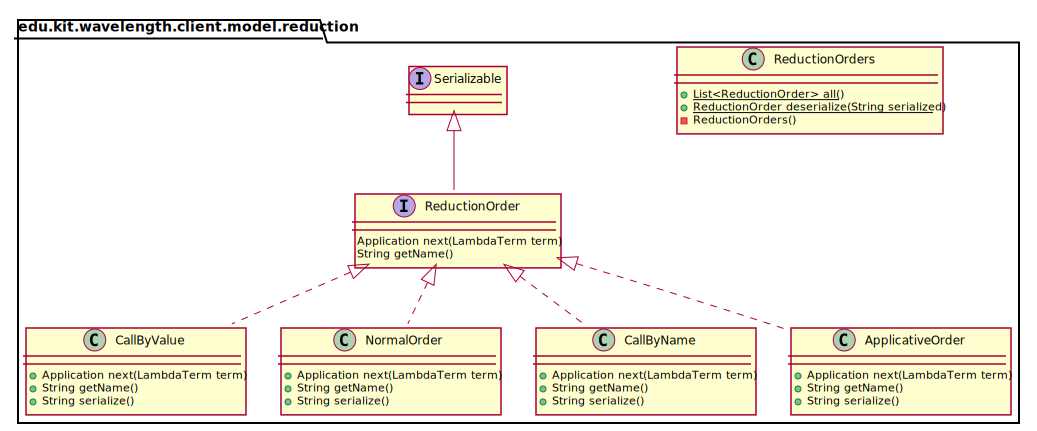
\includegraphics[width=\textwidth]{packageDiagrams/reductionPackage}
\end{figure}


\subsubsection{Class \texttt{ReductionOrders}}
\label{type:edu.kit.wavelength.client.model.reduction.ReductionOrders}
Static class giving access to all reduction orders known to the model.

Static methods:
\begin{itemize}
\item \texttt{List<\hyperref[type:edu.kit.wavelength.client.model.reduction.ReductionOrder]{ReductionOrder}> all()}

Returns an unmodifiable list of all reduction orders known to the model.

Returns: An unmodifiable list containing exactly one instance of all
 reduction orders known to the model

\item \texttt{\hyperref[type:edu.kit.wavelength.client.model.reduction.ReductionOrder]{ReductionOrder} deserialize(String serialized)}

Returns the reduction order represented by a given string.

\texttt{serialized}: A serialized reduction order

Returns: The reduction order the given string refers to, if known to the model

\end{itemize}

\subsubsection{Interface \texttt{ReductionOrder}}
\label{type:edu.kit.wavelength.client.model.reduction.ReductionOrder}
Extends: \texttt{\hyperref[type:edu.kit.wavelength.client.model.serialization.Serializable]{Serializable}}

Represents a reduction order for the untyped lambda calculus. A reduction
 order is a policy to determine the next reducible expression (redex) to be evaluated.

Methods:
\begin{itemize}
\item \texttt{\hyperref[type:edu.kit.wavelength.client.model.term.Application]{Application} next(\hyperref[type:edu.kit.wavelength.client.model.term.LambdaTerm]{LambdaTerm} term)}

Determines the next redex to be evaluated according to the reduction order.

\texttt{term}: The term whose next redex should be found.

Returns: \texttt{null} if there is no redex in the given term. Otherwise,
 the next redex to be evaluated.

\item \texttt{String getName()}

Returns the name of the reduction order, for example for display when
 selecting a reduction order in a user interface.

Returns: The name of the reduction order.

\end{itemize}

\subsubsection{Class \texttt{NormalOrder}}
\label{type:edu.kit.wavelength.client.model.reduction.NormalOrder}
Implements: \texttt{\hyperref[type:edu.kit.wavelength.client.model.reduction.ReductionOrder]{ReductionOrder}}

The normal reduction order for the untyped lambda calculus.
 
 The leftmost outermost redex is selected for reduction.

\subsubsection{Class \texttt{CallByValue}}
\label{type:edu.kit.wavelength.client.model.reduction.CallByValue}
Implements: \texttt{\hyperref[type:edu.kit.wavelength.client.model.reduction.ReductionOrder]{ReductionOrder}}

The call by value reduction order for the untyped lambda calculus.
 
 The leftmost outermost redex that is not enclosed by an abstraction
 and whose argument is a value (i.e. an abstraction) is selected for
 reduction.

\subsubsection{Class \texttt{CallByName}}
\label{type:edu.kit.wavelength.client.model.reduction.CallByName}
Implements: \texttt{\hyperref[type:edu.kit.wavelength.client.model.reduction.ReductionOrder]{ReductionOrder}}

The call by name reduction order for the untyped lambda calculus.
 
 The leftmost outermost redex that is not enclosed by an abstraction is
 selected for reduction.

\subsubsection{Class \texttt{ApplicativeOrder}}
\label{type:edu.kit.wavelength.client.model.reduction.ApplicativeOrder}
Implements: \texttt{\hyperref[type:edu.kit.wavelength.client.model.reduction.ReductionOrder]{ReductionOrder}}

The applicative reduction order for the untyped lambda calculus.

 The rightmost innermost redex is selected for reduction.

\subsection{Package \lstinline{edu.kit.wavelength.client.model.serialization}}
\label{pkg:edu.kit.wavelength.client.model.serialization}
The \texttt{\pkglnk{model.serialization}} package provides the \texttt{\lnk{Serializable}}
interface. Classes implementing this interface may be serialized into a string.

Since serialization in Wavelength is ad hoc by design, no entity is intended to hold
references to objects of type \texttt{\lnk{Serializable}}. It is provided merely to
ensure consistent naming of the \texttt{serialize} method. Deserialization occurs
in the classes providing the specific type (for example \texttt{\hyperref[type:edu.kit.wavelength.client.model.term.LambdaTerm]{LambdaTerm}}
or \texttt{\hyperref[type:edu.kit.wavelength.client.model.library.Libraries]{Libraries}} and its analogons in \texttt{\pkglnk{model.reduction}}
and \texttt{\pkglnk{model.output}}), which can be done, again, due to the ad hoc nature
of serialization, since each class knows which of its components it has serialized.


\subsubsection{Interface \texttt{Serializable}}
\label{type:edu.kit.wavelength.client.model.serialization.Serializable}
Implemented by objects that may be serialized into a string.

Methods:
\begin{itemize}
\item \texttt{String serialize()}

Creates a string designating the object's state.

Returns: A string designating the object's state from which it
 can be restored using a corresponding deserialization method

\end{itemize}

\subsection{Package \lstinline{edu.kit.wavelength.client.model.term}}
\label{pkg:edu.kit.wavelength.client.model.term}
Overview of \texttt{edu.kit.wavelength.client.model.term} with UML diagram.


\subsubsection{Interface \texttt{Visitor<T>}}
\label{type:edu.kit.wavelength.client.model.term.Visitor}
Represents a visitor that visits lambda terms and returns
 objects of a given type upon visiting a lambda term.

\texttt{<T>}: The type of object that is returned when visiting
 a term.

Methods:
\begin{itemize}
\item \texttt{T visitAbstraction(\hyperref[type:edu.kit.wavelength.client.model.term.Abstraction]{Abstraction} abs)}

Visit an abstraction.

\texttt{abs}: The abstraction to be visited

Returns: The return value of the visitor when visiting the given abstraction

\item \texttt{T visitApplication(\hyperref[type:edu.kit.wavelength.client.model.term.Application]{Application} app)}

Visit an application.

\texttt{app}: The application to be visited

Returns: The return value of the visitor when visiting the given application

\item \texttt{T visitBoundVariable(\hyperref[type:edu.kit.wavelength.client.model.term.BoundVariable]{BoundVariable} var)}

Visit a bound variable.

\texttt{var}: The bound variable to be visited

Returns: The return value of the visitor when visiting the given bound variable

\item \texttt{T visitFreeVariable(\hyperref[type:edu.kit.wavelength.client.model.term.FreeVariable]{FreeVariable} var)}

Visit a free variable.

\texttt{var}: The free variable to be visited

Returns: The return value of the visitor when visiting the given free variable

\item \texttt{T visitNamedTerm(\hyperref[type:edu.kit.wavelength.client.model.term.NamedTerm]{NamedTerm} term)}

Visit a named term.

\texttt{term}: The named term to be visited

Returns: The return value of the visitor when visiting the given named term

\item \texttt{T visitPartialApplication(\hyperref[type:edu.kit.wavelength.client.model.term.PartialApplication]{PartialApplication} app)}

Visit a partial application.

\texttt{app}: The partial application to be visited

Returns: The return value of the visitor when visiting the given partial application

\end{itemize}

\subsubsection{Abstract Class \texttt{TermTransformer}}
\label{type:edu.kit.wavelength.client.model.term.TermTransformer}
Implements: \texttt{\hyperref[type:edu.kit.wavelength.client.model.term.Visitor]{Visitor}}

A visitor that performs a transformation of some kind of a lambda term,
 automatically removing names if their inner term has been changed by
 the transformation.

\subsubsection{Class \texttt{SubstitutionVisitor}}
\label{type:edu.kit.wavelength.client.model.term.SubstitutionVisitor}
Extends: \texttt{\hyperref[type:edu.kit.wavelength.client.model.term.TermTransformer]{TermTransformer}}

A visitor that substitutes bound variables with a given De Bruijn
 index with a given substituent.

Constructors:
\begin{itemize}
\item \texttt{SubstitutionVisitor(int depth, \hyperref[type:edu.kit.wavelength.client.model.term.LambdaTerm]{LambdaTerm} substituent)}

Creates a new substitution visitor.

\texttt{depth}: The De Bruijn index that should be substituted

\texttt{substituent}: The term that should be substituted with

\end{itemize}

\subsubsection{Abstract Class \texttt{ResolvedNamesVisitor<T>}}
\label{type:edu.kit.wavelength.client.model.term.ResolvedNamesVisitor}
Implements: \texttt{\hyperref[type:edu.kit.wavelength.client.model.term.Visitor]{Visitor}}

A visitor that gives non-colliding names for bound variables.

\texttt{<T>}: The return value of the visitor

Methods:
\begin{itemize}
\item \texttt{protected abstract T visitBoundVariable(\hyperref[type:edu.kit.wavelength.client.model.term.BoundVariable]{BoundVariable} var, String resolvedName)}

Visit a bound variable with an additional non-colliding name for
 said variable.
 
 This method is provided merely for convenience, the given name
 will be the same as the one provided for the given abstraction.

\texttt{var}: The bound variable to be visited

\texttt{resolvedName}: The resolved name for the bound variable

Returns: The return value of the visitor upon visiting the given bound variable

\item \texttt{protected abstract T visitAbstraction(\hyperref[type:edu.kit.wavelength.client.model.term.Abstraction]{Abstraction} abs, String resolvedName)}

Visit an abstraction with an additional non-colliding name for
 its variable.

\texttt{abs}: The abstraction to be visited

\texttt{resolvedName}: The resolved name for the variable of this
 abstraction

Returns: The return value of the visitor upon visiting the given abstraction

\end{itemize}

\subsubsection{Abstract Class \texttt{PartialApplication}}
\label{type:edu.kit.wavelength.client.model.term.PartialApplication}
Implements: \texttt{\hyperref[type:edu.kit.wavelength.client.model.term.LambdaTerm]{LambdaTerm}}

Represents a term that consists of a library function that may be accelerated, as well as
 zero or more applications with arguments for said library function.

Constructors:
\begin{itemize}
\item \texttt{PartialApplication(String name, \hyperref[type:edu.kit.wavelength.client.model.term.LambdaTerm]{LambdaTerm} inner, int numParameters, \hyperref[type:edu.kit.wavelength.client.model.term.Visitor]{Visitor}<Boolean>[] checks)}

Creates a new partial application that has not yet bound any parameters

\texttt{name}: The name of the library function.

\texttt{inner}: The lambda term for the non-accelerated library function

\texttt{numParameters}: The number of parameters that the library function takes

\texttt{checks}: For each parameter, a visitor that checks whether the given parameter
 has the correct format for acceleration

\end{itemize}

Methods:
\begin{itemize}
\item \texttt{\hyperref[type:edu.kit.wavelength.client.model.term.LambdaTerm]{LambdaTerm} getRepresented()}

Returns the lambda term that this partial application represents.

Returns: The lambda term that this partial application represents

\item \texttt{String getName()}

Returns the name of the library function for the partial application.

Returns: The name of the library function for the partial application

\item \texttt{\hyperref[type:edu.kit.wavelength.client.model.term.LambdaTerm]{LambdaTerm} accept(\hyperref[type:edu.kit.wavelength.client.model.term.LambdaTerm]{LambdaTerm} nextParam)}

Accepts a new parameter for the partial application.
 
 If the parameter does not match the format that can be accelerated, returns a new term representing
 the unaccelerated application.
 
 If the parameter matches the format that can be accelerated, returns the result of the operation
 represented by the partial application if all parameters are now present, or a new PartialApplication
 representing the partial application including the given parameter.

\texttt{nextParam}: The parameter to be accepted

Returns: A lambda term for the partial application with the new parameter as described above

\item \texttt{protected abstract \hyperref[type:edu.kit.wavelength.client.model.term.LambdaTerm]{LambdaTerm} accelerate(\hyperref[type:edu.kit.wavelength.client.model.term.LambdaTerm]{LambdaTerm}[] parameters)}

Directly determine the result of the computation given all parameters.

\texttt{parameters}: The parameters for the computation

Returns: The result of the computation

\end{itemize}

\subsubsection{Class \texttt{NamedTerm}}
\label{type:edu.kit.wavelength.client.model.term.NamedTerm}
Implements: \texttt{\hyperref[type:edu.kit.wavelength.client.model.term.LambdaTerm]{LambdaTerm}}

Represents a term that has a name.

Constructors:
\begin{itemize}
\item \texttt{NamedTerm(String name, \hyperref[type:edu.kit.wavelength.client.model.term.LambdaTerm]{LambdaTerm} inner)}

Creates a new named term.

\texttt{name}: The name of the term

\texttt{inner}: The actual term that is being named

\end{itemize}

Methods:
\begin{itemize}
\item \texttt{\hyperref[type:edu.kit.wavelength.client.model.term.LambdaTerm]{LambdaTerm} getInner()}

Returns the term that the named term represents.

Returns: The term that the named term represents

\item \texttt{String getName()}

Returns the name of the term.

Returns: The name of the term

\end{itemize}

\subsubsection{Abstract Class \texttt{NameAgnosticVisitor<T>}}
\label{type:edu.kit.wavelength.client.model.term.NameAgnosticVisitor}
Implements: \texttt{\hyperref[type:edu.kit.wavelength.client.model.term.Visitor]{Visitor}}

A visitor that will treat a named term precisely like the term that
 it represents.

\texttt{<T>}: The return value of the visitor

\subsubsection{Interface \texttt{LambdaTerm}}
\label{type:edu.kit.wavelength.client.model.term.LambdaTerm}
Extends: \texttt{\hyperref[type:edu.kit.wavelength.client.model.serialization.Serializable]{Serializable}}

Represents a term in the untyped lambda calculus.

Static methods:
\begin{itemize}
\item \texttt{\hyperref[type:edu.kit.wavelength.client.model.term.LambdaTerm]{LambdaTerm} deserialize(String serialized)}

Creates a lambda term from its serialization.

\texttt{serialized}: The serialized representation of the lambda term

Returns: A lambda term that is equal to the term that was serialized

\end{itemize}

Methods:
\begin{itemize}
\item \texttt{<T> T acceptVisitor(\hyperref[type:edu.kit.wavelength.client.model.term.Visitor]{Visitor}<T> v)}

Accept a visitor by invoking the correct visit* method.

\texttt{v}: The visitor whose correct visit* method should be invoked

Returns: The return value of the invoked visit* method

\end{itemize}

\subsubsection{Class \texttt{IsRedexVisitor}}
\label{type:edu.kit.wavelength.client.model.term.IsRedexVisitor}
Extends: \texttt{\hyperref[type:edu.kit.wavelength.client.model.term.NameAgnosticVisitor]{NameAgnosticVisitor}}

A visitor that returns a boolean that is true iff the given
 lambda term represents a redex (possibly bound to one
 or more nested names).

\subsubsection{Class \texttt{IsAbstractionVisitor}}
\label{type:edu.kit.wavelength.client.model.term.IsAbstractionVisitor}
Extends: \texttt{\hyperref[type:edu.kit.wavelength.client.model.term.NameAgnosticVisitor]{NameAgnosticVisitor}}

A visitor that returns a boolean that is true iff the given
 lambda term represents an abstraction (possibly bound to one
 or more nested names).

\subsubsection{Class \texttt{FreeVariable}}
\label{type:edu.kit.wavelength.client.model.term.FreeVariable}
Implements: \texttt{\hyperref[type:edu.kit.wavelength.client.model.term.LambdaTerm]{LambdaTerm}}

Represents a free variable in the untyped lambda calculus.
 
 A free variable has a name. Unlike the name of the variable
 bound during an abstraction, this name is not a preferred name,
 but fixed, since it is free over the entire lambda term that
 is being represented. Changing this name would therefore
 change the lambda term.

Constructors:
\begin{itemize}
\item \texttt{FreeVariable(String name)}

Creates a new free variable term.

\texttt{name}: The name of the free variable being referenced

\end{itemize}

Methods:
\begin{itemize}
\item \texttt{String getName()}

Returns the name of the free variable.

Returns: The name of the free variable

\end{itemize}

\subsubsection{Class \texttt{BoundVariable}}
\label{type:edu.kit.wavelength.client.model.term.BoundVariable}
Implements: \texttt{\hyperref[type:edu.kit.wavelength.client.model.term.LambdaTerm]{LambdaTerm}}

Represents a bound variable in the untyped lambda calculus.
 
 It refers to its corresponding abstraction using its
 De Bruijn index.

Constructors:
\begin{itemize}
\item \texttt{BoundVariable(int deBruijnIndex)}

Creates a new bound variable term.

\texttt{deBruijnIndex}: The De Bruijn index of the term

\end{itemize}

Methods:
\begin{itemize}
\item \texttt{int getDeBruijnIndex()}

Returns the De Bruijn index of the variable.

Returns: The De Bruijn index

\end{itemize}

\subsubsection{Class \texttt{BetaReducer}}
\label{type:edu.kit.wavelength.client.model.term.BetaReducer}
Extends: \texttt{\hyperref[type:edu.kit.wavelength.client.model.term.TermTransformer]{TermTransformer}}

A visitor that transforms a lambda term by beta reducing a given
 redex.

Constructors:
\begin{itemize}
\item \texttt{BetaReducer(\hyperref[type:edu.kit.wavelength.client.model.term.Application]{Application} toReduce)}

Creates a new beta reducer that reduces the given redex

\texttt{toReduce}: The application that should be reduced.
 This must be a redex, otherwise an exception is thrown.

\end{itemize}

\subsubsection{Class \texttt{Application}}
\label{type:edu.kit.wavelength.client.model.term.Application}
Implements: \texttt{\hyperref[type:edu.kit.wavelength.client.model.term.LambdaTerm]{LambdaTerm}}

Represents an application in the untyped lambda calculus.
 
 An application has a left hand side and a right hand side,
 both of which may be arbitrary lambda terms.

Constructors:
\begin{itemize}
\item \texttt{Application(\hyperref[type:edu.kit.wavelength.client.model.term.LambdaTerm]{LambdaTerm} leftHandSide, \hyperref[type:edu.kit.wavelength.client.model.term.LambdaTerm]{LambdaTerm} rightHandSide)}

Creates a new application.

\texttt{leftHandSide}: The left hand side of the application

\texttt{rightHandSide}: The right hand side of the application

\end{itemize}

Methods:
\begin{itemize}
\item \texttt{\hyperref[type:edu.kit.wavelength.client.model.term.LambdaTerm]{LambdaTerm} getLeftHandSide()}

Returns the left hand side of the application.

Returns: The left hand side of the application

\item \texttt{\hyperref[type:edu.kit.wavelength.client.model.term.LambdaTerm]{LambdaTerm} getRightHandSide()}

Returns the right hand side of the application.

Returns: The right hand side of the application

\end{itemize}

\subsubsection{Class \texttt{Abstraction}}
\label{type:edu.kit.wavelength.client.model.term.Abstraction}
Implements: \texttt{\hyperref[type:edu.kit.wavelength.client.model.term.LambdaTerm]{LambdaTerm}}

Represents an abstraction in the untyped lambda calculus.
 
 An abstraction has an inner term and a preferred name for the
 variable it abstracts. When displaying the abstraction, a different
 name may be used, since terms referring to this abstraction
 will use De Bruijn indices to do so.

Constructors:
\begin{itemize}
\item \texttt{Abstraction(String preferredName, \hyperref[type:edu.kit.wavelength.client.model.term.LambdaTerm]{LambdaTerm} inner)}

Creates a new abstraction.

\texttt{preferredName}: The preferred name for the variable that is abstracted

\texttt{inner}: The lambda term that the abstraction encloses

\end{itemize}

Methods:
\begin{itemize}
\item \texttt{String getPreferredName()}

Gets the preferred name for the abstracted variable.

Returns: The preferred name

\item \texttt{\hyperref[type:edu.kit.wavelength.client.model.term.LambdaTerm]{LambdaTerm} getInner()}

Gets the inner term of the abstraction.

Returns: The term that this abstraction encloses

\end{itemize}

\subsection{Package \lstinline{edu.kit.wavelength.client.model.term.parsing}}
\label{pkg:edu.kit.wavelength.client.model.term.parsing}
Overview of \texttt{edu.kit.wavelength.client.model.term.parsing} with UML diagram.


\subsubsection{Class \texttt{Tokeniser}}
\label{type:edu.kit.wavelength.client.model.term.parsing.Tokeniser}
The Tokeniser class is used during the first step of the parsing process to turn the entered input into a sequence of Tokens.

Methods:
\begin{itemize}
\item \texttt{\hyperref[type:edu.kit.wavelength.client.model.term.parsing.Token]{Token}[] tokenise(String input)}

Divides a sequence of characters into Tokens.

\texttt{input}: The String to divide into tokens

Returns: An array containing all tokens

\end{itemize}

\subsubsection{Class \texttt{Token}}
\label{type:edu.kit.wavelength.client.model.term.parsing.Token}
Token objects are used by both the Tokeniser and the Parser during the construction of an lambda-term from an input String.
 Each token contains a part of the input String which can be accessed through this class' interface.

Constructors:
\begin{itemize}
\item \texttt{Token(String content)}

Creates a new Token containing the entered String.

\texttt{content}: The String to be stored in the Token

\end{itemize}

Methods:
\begin{itemize}
\item \texttt{String getContent()}

Used to access the String that makes up the token.

Returns: The String making up the token

\end{itemize}

\subsubsection{Class \texttt{Parser}}
\label{type:edu.kit.wavelength.client.model.term.parsing.Parser}
This class is used to convert an input String into a lambda term object.
 If any libraries terms are used in the input, the necessary libraries have to passed to the Parser through its constructor.

Constructors:
\begin{itemize}
\item \texttt{Parser(List<\hyperref[type:edu.kit.wavelength.client.model.library.Library]{Library}> libraries)}

Initializes a new parser.

\texttt{libraries}: The libraries to be taken into consideration during parsing

\end{itemize}

Methods:
\begin{itemize}
\item \texttt{\hyperref[type:edu.kit.wavelength.client.model.term.LambdaTerm]{LambdaTerm} parse(String input)}

Parses the input text representation of a Lambda-term and turns it into a LambdaTerm object if successful.

\texttt{input}: The String to parse.

Returns: The parsed LambdaTerm object

\end{itemize}

\subsubsection{Class \texttt{ParseException}}
\label{type:edu.kit.wavelength.client.model.term.parsing.ParseException}
Extends: \texttt{Exception}

An exception used to indicate an error during the parsing of an entered lambda term.

Constructors:
\begin{itemize}
\item \texttt{ParseException(String message, int row, int column)}

Creates a new ParseException with the entered parameters.

\texttt{message}: A message to the user describing the error causing the exception

\texttt{row}: The row containing the source of this exception

\texttt{column}: The row containing the source of this exception

\end{itemize}

Methods:
\begin{itemize}
\item \texttt{int getRow()}

Gets the row in which the error causing this exception occurred.

Returns: The row in which the error occurred

\item \texttt{int getColumn()}

Gets the column in which the error causing this exception occurred.

Returns: The column in which the error occurred

\end{itemize}

\subsection{Package \lstinline{edu.kit.wavelength.client.view.action}}
\label{pkg:edu.kit.wavelength.client.view.action}
% Leave me here, I am neecessary for \lnk to work.
% See the wiki page "Entwurfsdokument"
\renewcommand\pkg{edu.kit.wavelength.client.view.action}

Overview of \texttt{\pkg} with UML diagram.


\subsubsection{Class \texttt{UseShare}}
\label{type:edu.kit.wavelength.client.view.action.UseShare}
Implements: \texttt{\hyperref[type:edu.kit.wavelength.client.view.action.Action]{Action}}

This action toggles the permalink panel. The permalink encodes the current
 input, output and settings.

Constructors:
\begin{itemize}
\item \texttt{UseShare(\hyperref[type:edu.kit.wavelength.client.view.URLSerializer]{URLSerializer} serializer)}

Constructs a new action handler for the permalink request.

\texttt{serializer}: The instance to delegate the serialization process to.

\end{itemize}

Methods:
\begin{itemize}
\item \texttt{void run()}

Hides the share panel if it is currently shown, otherwise generates the
 permalink that encodes the current input, output and settings.

\end{itemize}

\subsubsection{Class \texttt{UnpauseExecution}}
\label{type:edu.kit.wavelength.client.view.action.UnpauseExecution}
Implements: \texttt{\hyperref[type:edu.kit.wavelength.client.view.action.Action]{Action}}

This action continues the paused reduction process.

Methods:
\begin{itemize}
\item \texttt{void run()}

Continues the paused reduction process, disables the step-by-step buttons and
 the option menus.

\end{itemize}

\subsubsection{Class \texttt{Stop}}
\label{type:edu.kit.wavelength.client.view.action.Stop}
Implements: \texttt{\hyperref[type:edu.kit.wavelength.client.view.action.Action]{Action}}

This action stops the currently running reduction process and re-enables all
 input related components.

Methods:
\begin{itemize}
\item \texttt{void run()}

Re-enables the editor and all option menus and blocks all buttons except the
 run button. Does not clear the output view.

\end{itemize}

\subsubsection{Class \texttt{StepManually}}
\label{type:edu.kit.wavelength.client.view.action.StepManually}
Implements: \texttt{\hyperref[type:edu.kit.wavelength.client.view.action.Action]{Action}}

Action that initiates a manual step on a particular redex in an output view.

Constructors:
\begin{itemize}
\item \texttt{StepManually(\hyperref[type:edu.kit.wavelength.client.model.term.Application]{Application} redex)}

Creates the action with the redex to apply when the user clicks on a
 redex.

\texttt{redex}: The redex to apply

\end{itemize}

Methods:
\begin{itemize}
\item \texttt{void run()}

Delegates the step to the Executor.

\end{itemize}

\subsubsection{Class \texttt{StepForward}}
\label{type:edu.kit.wavelength.client.view.action.StepForward}
Implements: \texttt{\hyperref[type:edu.kit.wavelength.client.view.action.Action]{Action}}

This action requests and displays the next reduction step of the current
 execution.

Methods:
\begin{itemize}
\item \texttt{void run()}

Requests and displays the next reduction step.

\end{itemize}

\subsubsection{Class \texttt{StepByStep}}
\label{type:edu.kit.wavelength.client.view.action.StepByStep}
Implements: \texttt{\hyperref[type:edu.kit.wavelength.client.view.action.Action]{Action}}

This class starts a new reduction process by requesting only the first
 reduction step.

Methods:
\begin{itemize}
\item \texttt{void run()}

Reads the users input and all required options from the option menus and
 delegates the reduction process to the Executor. Disables
 the editor and some option menus and toggles the buttons accordingly.

\end{itemize}

\subsubsection{Class \texttt{StepBackward}}
\label{type:edu.kit.wavelength.client.view.action.StepBackward}
Implements: \texttt{\hyperref[type:edu.kit.wavelength.client.view.action.Action]{Action}}

This class removes the last shown reduction step from the output.

Methods:
\begin{itemize}
\item \texttt{void run()}

Removes the last shown step from the output.

\end{itemize}

\subsubsection{Class \texttt{SetReductionOrder}}
\label{type:edu.kit.wavelength.client.view.action.SetReductionOrder}
Implements: \texttt{\hyperref[type:edu.kit.wavelength.client.view.action.Action]{Action}}

This action changes the reduction order for the further execution.

Methods:
\begin{itemize}
\item \texttt{void run()}

Changes the reduction order to the selected one.

\end{itemize}

\subsubsection{Class \texttt{SelectExportFormat}}
\label{type:edu.kit.wavelength.client.view.action.SelectExportFormat}
Implements: \texttt{\hyperref[type:edu.kit.wavelength.client.view.action.Action]{Action}}

This action displays the currently displayed output in the selected export
 format in a pop up export window.

Constructors:
\begin{itemize}
\item \texttt{SelectExportFormat(\hyperref[type:edu.kit.wavelength.client.view.export.Export]{Export} exportFormat)}

Constructs a new action handler for the selection of an export format.

\texttt{exportFormat}: The export format the user chose.

\end{itemize}

Methods:
\begin{itemize}
\item \texttt{void run()}

Gets the representation of the current output in the selected export format
 and writes it into the export output window. Displays this window and disables
 user interaction with all elements, except the export window.

\end{itemize}

\subsubsection{Class \texttt{SelectExercise}}
\label{type:edu.kit.wavelength.client.view.action.SelectExercise}
Implements: \texttt{\hyperref[type:edu.kit.wavelength.client.view.action.Action]{Action}}

This action will try to load a new exercise and alerts the user that the
 content of the Editor would be overwritten.

Constructors:
\begin{itemize}
\item \texttt{SelectExercise(\hyperref[type:edu.kit.wavelength.client.view.exercise.Exercise]{Exercise} exercise)}

Constructs a new action handler for the selection of an exercise.

\texttt{exercise}: the selected Exercise that should be loaded

\end{itemize}

Methods:
\begin{itemize}
\item \texttt{void run()}

Opens a PopupWindow if the content of the editor would be overwritten.
 Allows the user to choose whether he wants to continue.
 Otherwise just loads the selected exercise.

\end{itemize}

\subsubsection{Class \texttt{RunNewExecution}}
\label{type:edu.kit.wavelength.client.view.action.RunNewExecution}
Implements: \texttt{\hyperref[type:edu.kit.wavelength.client.view.action.Action]{Action}}

This class starts a new reduction process and sets the view accordingly.

Methods:
\begin{itemize}
\item \texttt{void run()}

Reads the users input and all required options from the option menus and
 delegates the reduction process to the Executor.
 Disables the editor and option menus and toggles the play button.

\end{itemize}

\subsubsection{Class \texttt{Pause}}
\label{type:edu.kit.wavelength.client.view.action.Pause}
Implements: \texttt{\hyperref[type:edu.kit.wavelength.client.view.action.Action]{Action}}

This class pauses the currently running execution process and allows the user
 to now navigate through the reduction process himself.

Methods:
\begin{itemize}
\item \texttt{void run()}

Pause the running execution and enable the step-by-step buttons. Also allow
 output window interactions and enable the reduction order option.

\end{itemize}

\subsubsection{Class \texttt{LoadExercise}}
\label{type:edu.kit.wavelength.client.view.action.LoadExercise}
Implements: \texttt{\hyperref[type:edu.kit.wavelength.client.view.action.Action]{Action}}

This class changes the view from standard input to exercise view to display
 the selected exercise.

Constructors:
\begin{itemize}
\item \texttt{LoadExercise(\hyperref[type:edu.kit.wavelength.client.view.exercise.Exercise]{Exercise} exercise)}

Constructs a new action for changing the UI from standard input view to
 exercise view.

\texttt{exercise}: The selected Exercise that should be displayed to the user

\end{itemize}

Methods:
\begin{itemize}
\item \texttt{void run()}

Reduces the editors width and displays the task in the enabled task view
 window. Also shows buttons for exiting this exercise view and for displaying
 the sample solution.

\end{itemize}

\subsubsection{Class \texttt{HideComponent}}
\label{type:edu.kit.wavelength.client.view.action.HideComponent}
Implements: \texttt{\hyperref[type:edu.kit.wavelength.client.view.action.Action]{Action}}

This action generalizes interaction with UI components that do nothing but
 being shown or hid.

Methods:
\begin{itemize}
\item \texttt{void run()}

Hides the given component if currently displayed, displays it otherwise.

\end{itemize}

\subsubsection{Class \texttt{ExitExerciseMode}}
\label{type:edu.kit.wavelength.client.view.action.ExitExerciseMode}
Implements: \texttt{\hyperref[type:edu.kit.wavelength.client.view.action.Action]{Action}}

This action will try to exit the exercise mode and alerts the user when
 contents of the editor would be overwritten. Otherwise it changes the view
 from exercise view to standard input view.

Methods:
\begin{itemize}
\item \texttt{void run()}

Opens a popup window if the editor contains code that would be overwritten.
 If this is not the case this method changes the view to standard input view.

\end{itemize}

\subsubsection{Class \texttt{EnterDefaultMode}}
\label{type:edu.kit.wavelength.client.view.action.EnterDefaultMode}
Implements: \texttt{\hyperref[type:edu.kit.wavelength.client.view.action.Action]{Action}}

This class changes the view from exercise mode view to standard input view.

Methods:
\begin{itemize}
\item \texttt{void run()}

Resizes the editor window to full width, hides the solution and task windows
 and hides the buttons for exiting and showing the solution.

\end{itemize}

\subsubsection{Class \texttt{CopyExport}}
\label{type:edu.kit.wavelength.client.view.action.CopyExport}
Implements: \texttt{\hyperref[type:edu.kit.wavelength.client.view.action.Action]{Action}}

This action class copies the generated and displayed export output to the
 users clipboard.

Methods:
\begin{itemize}
\item \texttt{void run()}

Reads the current export output from the export output window and copies it
 to the users clipboard.

\end{itemize}

\subsubsection{Class \texttt{CloseExport}}
\label{type:edu.kit.wavelength.client.view.action.CloseExport}
Implements: \texttt{\hyperref[type:edu.kit.wavelength.client.view.action.Action]{Action}}

This class closes the pop up window that displays the generated export
 output. It re-enables the UI after the window is closed.

Methods:
\begin{itemize}
\item \texttt{void run()}

Hides the export output window and re-enables the UI.

\end{itemize}

\subsubsection{Interface \texttt{Action}}
\label{type:edu.kit.wavelength.client.view.action.Action}
The Action interface encapsulates all events that can occur from the user
 interacting with the UI.
 
 An Action class is the event handler for one UI event. It is triggered by
 interacting with the dedicated UI element.

Methods:
\begin{itemize}
\item \texttt{void run()}

Called when the Action is triggered.

\end{itemize}

\subsection{Package \lstinline{edu.kit.wavelength.client.view.api}}
\label{pkg:edu.kit.wavelength.client.view.api}
The \texttt{api} package contains a collection of interfaces for the \texttt{\pkglnk{view.webui.components}} package.

%TODO hier hätte mal ein schöner Abschnitt zur Entkopplung oder Abstraktionsebene hinkommen können 
%TODO aber das ist schon lang geschmolzener Schnee von Gestern :(
The interfaces provide consistent naming of methods. This is especially important for the adapter classes from the
\texttt{\pkglnk{view.webui.components}}.

\begin{figure}[H]
	\centering
	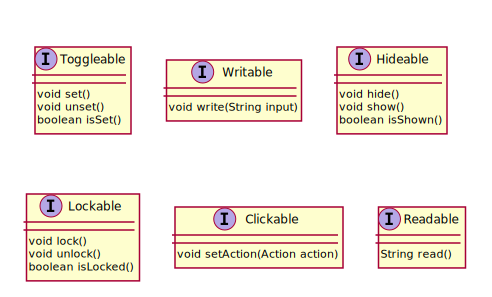
\includegraphics[width=\textwidth]{packageDiagrams/apiPackage}
\end{figure}


\subsubsection{Interface \texttt{Writable}}
\label{type:edu.kit.wavelength.client.view.api.Writable}
A Writable is a View whose content can be overwritten.
 
 By implementing this interface a View component provides a means of writing
 its content.

Methods:
\begin{itemize}
\item \texttt{void write(String input)}

Writes content into this element.

\texttt{input}: A String representation of the designated new content

\end{itemize}

\subsubsection{Interface \texttt{Toggleable}}
\label{type:edu.kit.wavelength.client.view.api.Toggleable}
Expresses that a view the view has a state that can be set and unset (e.g. a checkbox)

Methods:
\begin{itemize}
\item \texttt{void set()}

Sets the state.

\item \texttt{void unset()}

Unsets the state.

\item \texttt{boolean isSet()}

Checks whether the state is set.

Returns: whether the state is set.

\end{itemize}

\subsubsection{Interface \texttt{Readable}}
\label{type:edu.kit.wavelength.client.view.api.Readable}
A Readable is a View whose content can be read.
 
 By implementing this interface a View component provides a means of reading
 its content.

Methods:
\begin{itemize}
\item \texttt{String read()}

Returns the content of a View as a String.

Returns: String representation of a View's content.

\end{itemize}

\subsubsection{Interface \texttt{Lockable}}
\label{type:edu.kit.wavelength.client.view.api.Lockable}
A Lockable is a view that can be locked and unlocked.

 Being locked means that an object is still visible but cannot react to any event.
 By unlocking an object it can react to events again.

Methods:
\begin{itemize}
\item \texttt{void lock()}

Lock this element, disabling actions on the element.

\item \texttt{void unlock()}

Unlock this element, enabling actions on the element.

\item \texttt{boolean isLocked()}

Checks whether the view is locked right now.

Returns: whether the view is locked

\end{itemize}

\subsubsection{Interface \texttt{Hideable}}
\label{type:edu.kit.wavelength.client.view.api.Hideable}
A Hideable is a View that can be hidden or shown.
 
 Being hidden means that an element is still there but not visible on the UI.

Methods:
\begin{itemize}
\item \texttt{void hide()}

Makes this element invisible.

\item \texttt{void show()}

Makes this element visible.

\item \texttt{boolean isShown()}

Checks whether this element is visible.

Returns: true if visible

\end{itemize}

\subsubsection{Interface \texttt{Clickable}}
\label{type:edu.kit.wavelength.client.view.api.Clickable}
This interface is intended to enable Buttons to have their associated
 \texttt{Action} set after creation.

Methods:
\begin{itemize}
\item \texttt{void setAction(\hyperref[type:edu.kit.wavelength.client.view.action.Action]{Action} action)}

Sets the current Action.

\texttt{action}: action that this can invoke

\end{itemize}

\subsection{Package \lstinline{edu.kit.wavelength.client.view}}
\label{pkg:edu.kit.wavelength.client.view}
Overview of \texttt{edu.kit.wavelength.client.view} with UML diagram.


\subsubsection{Class \texttt{URLSerializer}}
\label{type:edu.kit.wavelength.client.view.URLSerializer}
Serializes a serializable into an URL every N milliseconds.

Constructors:
\begin{itemize}
\item \texttt{URLSerializer(\hyperref[type:edu.kit.wavelength.client.model.serialization.Serializable]{Serializable} serializable, List<\hyperref[type:edu.kit.wavelength.client.view.SerializationObserver]{SerializationObserver}> serializationOutputs, int pollingDelayMS)}

Creates a new serializer.

\texttt{serializable}: Serializable to serialize

\texttt{serializationOutputs}: Observers to update with new serialized URL

\texttt{pollingDelayMS}: Delay between every serialization iteration. The serializable may change, so we poll it.

\end{itemize}

Methods:
\begin{itemize}
\item \texttt{void startPolling()}

Starts polling (serializing) the serializable.

\item \texttt{boolean serialize()}

Executes a serialization instantly.

Returns: whether the serializer will continue to poll after this call

\end{itemize}

\subsubsection{Interface \texttt{SerializationObserver}}
\label{type:edu.kit.wavelength.client.view.SerializationObserver}
Observer that receives updates with the most recent serialized URL.

Methods:
\begin{itemize}
\item \texttt{void updateSerialized(String s)}

Updates the observer.

\texttt{s}: - serialized URL

\end{itemize}

\subsubsection{Class \texttt{App}}
\label{type:edu.kit.wavelength.client.view.App}
Implements: \texttt{\hyperref[type:edu.kit.wavelength.client.model.serialization.Serializable]{Serializable}}

This class handles the current state of the application and the currently
 displayed output. The initial state is the Input state and the output is
 empty when the application is started.

Static methods:
\begin{itemize}
\item \texttt{\hyperref[type:edu.kit.wavelength.client.view.App]{App} get()}

Gets a singleton instance of App.

Returns: instance

\item \texttt{void set(\hyperref[type:edu.kit.wavelength.client.view.App]{App} a)}

Sets the singleton instance of App for testing.

\texttt{a}: instance to set

\end{itemize}

Methods:
\begin{itemize}
\item \texttt{\hyperref[type:edu.kit.wavelength.client.view.webui.component.TextField]{TextField} sharePanel()}

Gets the panel that contains the URL to play back the state of the application.

Returns: panel

\item \texttt{\hyperref[type:edu.kit.wavelength.client.view.webui.component.PopUpWindow]{PopUpWindow} exportWindow()}

Gets the window that shows exported output.

Returns: window

\item \texttt{\hyperref[type:edu.kit.wavelength.client.view.webui.component.ImageButton]{ImageButton} mainMenuButton()}

Gets the button that is used to open the main menu.

Returns: button

\item \texttt{\hyperref[type:edu.kit.wavelength.client.view.webui.component.Editor]{Editor} editor()}

Gets the editor.

Returns: editor

\item \texttt{\hyperref[type:edu.kit.wavelength.client.view.webui.component.OptionBox]{OptionBox} outputFormatBox()}

Gets the option box that allows the user to choose which output format to use.

Returns: box

\item \texttt{\hyperref[type:edu.kit.wavelength.client.view.webui.component.OptionBox]{OptionBox} reductionOrderBox()}

Gets the option box that allows the user to choose which reduction order to use.

Returns: box

\item \texttt{\hyperref[type:edu.kit.wavelength.client.view.webui.component.OptionBox]{OptionBox} outputSizeBox()}

Gets the option box that allows the user to choose which output size to use.

Returns: box

\item \texttt{\hyperref[type:edu.kit.wavelength.client.view.webui.component.ImageButton]{ImageButton} stepBackwardButton()}

Gets the button that can be used to play back to the previous displayed term.

Returns: button

\item \texttt{\hyperref[type:edu.kit.wavelength.client.view.webui.component.ImageButton]{ImageButton} stepByStepModeButton()}

Gets the button that can be used to initiate step by step reduction before execution.

Returns: button

\item \texttt{\hyperref[type:edu.kit.wavelength.client.view.webui.component.ImageButton]{ImageButton} stepForwardButton()}

Gets the button that can be used to initiate the next reduction by the currently selected reduction order.

Returns: button

\item \texttt{\hyperref[type:edu.kit.wavelength.client.view.webui.component.ImageButton]{ImageButton} terminateButton()}

Gets the button that can be used to terminate the reduction.

Returns: button

\item \texttt{\hyperref[type:edu.kit.wavelength.client.view.webui.component.ImageButton]{ImageButton} runButton()}

Gets the button that can be used to initiate the execution, automatically reducing the input with the given options

Returns: button

\item \texttt{\hyperref[type:edu.kit.wavelength.client.view.webui.component.ImageButton]{ImageButton} pauseButton()}

Gets the button that can be used to transition from the automatic execution to the step by step mode.

Returns: button

\item \texttt{\hyperref[type:edu.kit.wavelength.client.view.webui.component.TreeOutput]{TreeOutput} treeOutput()}

Gets the output that displays terms as trees.

Returns: output

\item \texttt{\hyperref[type:edu.kit.wavelength.client.view.webui.component.UnicodeOutput]{UnicodeOutput} unicodeOutput()}

Gets the output that displays terms with unicode text.

Returns: output

\item \texttt{\hyperref[type:edu.kit.wavelength.client.view.webui.component.ImageButton]{ImageButton} exportButton()}

Gets the button that can be used to open the menu that allows the user to choose an export format.

Returns: button

\item \texttt{\hyperref[type:edu.kit.wavelength.client.view.webui.component.ImageButton]{ImageButton} shareButton()}

Gets the button that can be used to toggle the panel that displays the serialized URL.

Returns: button

\item \texttt{List<\hyperref[type:edu.kit.wavelength.client.view.webui.component.Checkbox]{Checkbox}> libraryBoxes()}

Gets all checkboxes that can be used to enable libraries.

Returns: library checkboxes

\item \texttt{List<\hyperref[type:edu.kit.wavelength.client.view.webui.component.TextButton]{TextButton}> exerciseButtons()}

Gets all buttons that can be used to load an exercise.

Returns: exercise buttons

\item \texttt{List<\hyperref[type:edu.kit.wavelength.client.view.webui.component.TextButton]{TextButton}> exportFormatButtons()}

Gets all buttons that can be used to load the output into the export window with the given export format specified by the button.

Returns: export format buttons

\item \texttt{\hyperref[type:edu.kit.wavelength.client.view.execution.Executor]{Executor} executor()}

Gets the wrapper that controls the reduction of lambda terms.

Returns: Executor

\end{itemize}

\subsection{Package \lstinline{edu.kit.wavelength.client.view.execution}}
\label{pkg:edu.kit.wavelength.client.view.execution}
The package \texttt{view.execution} holds the \texttt{\lnk{Executor}}, which adapts a \texttt{\hyperref[type:edu.kit.wavelength.client.model.ExecutionEngine]{ExecutionEngine}}.
This adaption is necessary because the reduction of a lambda term is concurrent with the UI interaction itself. 
As GWT runs in a single threaded browser environment, it has its own concurrency mechanism: A \texttt{Scheduler} that allows one to schedule a specific action at the end of the event loop of the browser.
As a result of this the Executor schedules one reduction step at the end of every event loop iteration and provides methods to control this concurrent execution.
The package also contains an \texttt{\lnk{ExecutionObserver}}, which is used by the \texttt{\lnk{Executor}} to push reduced terms that are intended to be displayed in the \texttt{\pkglnk{view}} to observers observing it.

\begin{figure}[H]
	\centering
	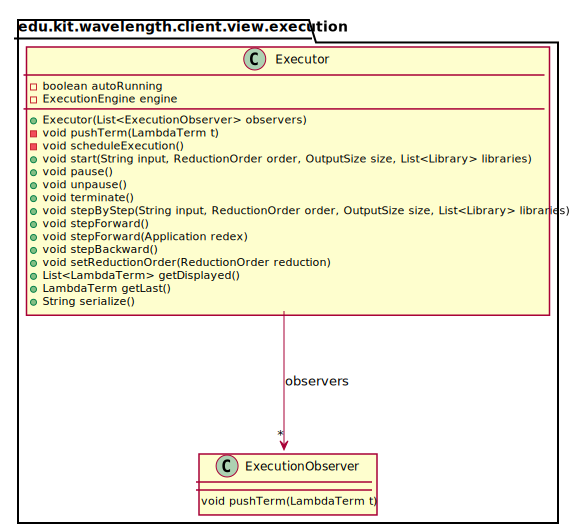
\includegraphics[width=\textwidth]{packageDiagrams/executionPackage}
\end{figure}


\subsubsection{Class \texttt{Executor}}
\label{type:edu.kit.wavelength.client.view.execution.Executor}
Concurrently reduces lambda terms.

Constructors:
\begin{itemize}
\item \texttt{Executor(List<\hyperref[type:edu.kit.wavelength.client.view.execution.ExecutionObserver]{ExecutionObserver}> observers)}

Creates a new Executor.

\texttt{observers}: Observers to update with reduced lambda terms

\end{itemize}

Methods:
\begin{itemize}
\item \texttt{void start(String input, \hyperref[type:edu.kit.wavelength.client.model.reduction.ReductionOrder]{ReductionOrder} order, \hyperref[type:edu.kit.wavelength.client.model.output.OutputSize]{OutputSize} size, List<\hyperref[type:edu.kit.wavelength.client.model.library.Library]{Library}> libraries)}

Starts the automatic execution of the input, parsing the term and then reducing it.

\texttt{input}: code to parse and reduce

\texttt{order}: order with which to reduce

\texttt{size}: which terms to push to observers

\texttt{libraries}: libraries to consider when parsing

\item \texttt{void pause()}

Pauses the automatic execution, transitioning into the step by step mode.

\item \texttt{void unpause()}

Unpauses the automatic execution, transitioning from step by step mode into automatic execution.

\item \texttt{void terminate()}

Terminates the step by step- and automatic execution.

\item \texttt{void stepByStep(String input, \hyperref[type:edu.kit.wavelength.client.model.reduction.ReductionOrder]{ReductionOrder} order, \hyperref[type:edu.kit.wavelength.client.model.output.OutputSize]{OutputSize} size, List<\hyperref[type:edu.kit.wavelength.client.model.library.Library]{Library}> libraries)}

Initiates the step by step execution, allowing the caller to choose the next step.

\texttt{input}: code to parse and execute

\texttt{order}: order with which to reduce

\texttt{size}: which terms to push to observers

\texttt{libraries}: libraries to consider when parsing

\item \texttt{void stepForward()}

Executes a single reduction of the current lambda term.

\item \texttt{void stepForward(\hyperref[type:edu.kit.wavelength.client.model.term.Application]{Application} redex)}

Executes a single reduction of the supplied redex.

\texttt{redex}: The redex to be evaluated. Must be a redex, otherwise
 an exception is thrown

\item \texttt{void stepBackward()}

Reverts to the previously output lambda term.

\item \texttt{void setReductionOrder(\hyperref[type:edu.kit.wavelength.client.model.reduction.ReductionOrder]{ReductionOrder} reduction)}

Changes the active reduction order to the entered one.

\texttt{reduction}: The new reduction order.

\item \texttt{List<\hyperref[type:edu.kit.wavelength.client.model.term.LambdaTerm]{LambdaTerm}> getDisplayed()}

Returns a list of all lambda terms that have been displayed.

Returns: A list of all lambda terms that have been displayed

\item \texttt{\hyperref[type:edu.kit.wavelength.client.model.term.LambdaTerm]{LambdaTerm} getLast()}

Returns the last lambda term that has been displayed.

Returns: The last lambda term that has been displayed

\item \texttt{String serialize()}

Serializes the Executor by serializing its ExecutionEngine.

Returns: The Executor serialized String representation

\end{itemize}

\subsubsection{Interface \texttt{ExecutionObserver}}
\label{type:edu.kit.wavelength.client.view.execution.ExecutionObserver}
Observer that receives reduced terms. Necessary because Executor is concurrent with UI.

Methods:
\begin{itemize}
\item \texttt{void pushTerm(\hyperref[type:edu.kit.wavelength.client.model.term.LambdaTerm]{LambdaTerm} t)}

Pushes the most recent displayed term.

\texttt{t}: term

\end{itemize}

\subsection{Package \lstinline{edu.kit.wavelength.client.view.exercise}}
\label{pkg:edu.kit.wavelength.client.view.exercise}
The \texttt{\pkglnk{view.exercise}} package contains the applications exercise system:

The \texttt{\lnk{Exercise}} interface specifies that exercises consist of a name, a task, a solution and (optional) predefined variables.
The \texttt{\lnk{ConcreteExercise}} class gives an implementation allowing for a simple generation of exercises.
Note that exercises use String representations of $\lambda$-Terms which must be transformed to \texttt{\hyperref[type:edu.kit.wavelength.client.model.term.LambdaTerm]{LambdaTerm}} objects when used.

The \texttt{\lnk{Exercises}} class static has only one method which statically returns a list of all available exercises.

\begin{figure}[H]
	\centering
	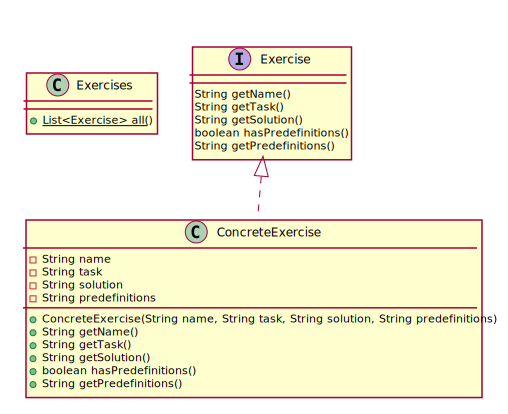
\includegraphics[width=0.8\textwidth]{packageDiagrams/exercisePackage}
\end{figure}



\subsubsection{Class \texttt{Exercises}}
\label{type:edu.kit.wavelength.client.view.exercise.Exercises}
Static class giving access to all available exercises.

Static methods:
\begin{itemize}
\item \texttt{List<\hyperref[type:edu.kit.wavelength.client.view.exercise.Exercise]{Exercise}> all()}

Returns an unmodifiable list of all available exercises.

Returns: An unmodifiable list that contains exactly one instance of every
         available exercise.

\end{itemize}

\subsubsection{Interface \texttt{Exercise}}
\label{type:edu.kit.wavelength.client.view.exercise.Exercise}
An exercise consists of a task specifying what the User is supposed to do and
 a solution specifying what the result should look like. Additionally
 exercises may provide a basis for a given task. In order to evaluate a
 solution there are some test cases provided as Strings, meaning that they
 need to be evaluated by the \texttt{ExecutionEngine} and matched against a
 possible solution.

Methods:
\begin{itemize}
\item \texttt{String getName()}

Gets the name of the exercise.

Returns: name

\item \texttt{String getTask()}

Returns the explanation of the exercise.

Returns: The task

\item \texttt{String getSolution()}

Returns the sample solution. Note that this may not be the only possible
 solution.

Returns: the solution

\item \texttt{boolean hasPredefinitions()}

Returns whether this has predefined code or not.

Returns: \texttt{true} if this Exercise has predefined code

\item \texttt{String getPredefinitions()}

Returns initial definitions that are supposed to be of help for the User.
 Note that this may be empty.

Returns: the predefined code

\end{itemize}

\subsubsection{Class \texttt{ConcreteExercise}}
\label{type:edu.kit.wavelength.client.view.exercise.ConcreteExercise}
Implements: \texttt{\hyperref[type:edu.kit.wavelength.client.view.exercise.Exercise]{Exercise}}

This class is a concrete implementation of the \texttt{Exercise} interface.
 The needed method's return values are set in the constructor.

Constructors:
\begin{itemize}
\item \texttt{ConcreteExercise(String name, String task, String solution, String predefinitions)}

Creates a new Exercise.

\texttt{name}: - name of the exercise

\texttt{task}: - problem task to display

\texttt{solution}: - intended solution for the problem

\texttt{predefinitions}: - initial code to load into the editor

\end{itemize}

\subsection{Package \lstinline{edu.kit.wavelength.client.view.export}}
\label{pkg:edu.kit.wavelength.client.view.export}
The \texttt{export} package provides the classes used by the application to transform given \texttt{\hyperref[type:edu.kit.wavelength.client.model.term.LambdaTerm]{LambdaTerms}} into a String representation depending on the selected format. Also the \texttt{export} package contains a \texttt{\lnk{Exports}} class that provides information about the available export formats. 

All format classes implement the interface \texttt{\lnk{Export}}. The representation of given \texttt{\hyperref[type:edu.kit.wavelength.client.model.term.LambdaTerm]{LambdaTerm}} can thus be requested via a unique method. 
The second method of the interface returns the name of the export format to the caller.
Since these classes just transform the given terms, it is not guaranteed that the generated representation is executable. This concerns mainly the classes \texttt{\lnk{HaskellExport}} and \texttt{\lnk{LispExport}}.

All available export formats can be requested by calling the \texttt{\lnk{Exports}} class. Its single method returns a collection of the export format classes.  

\begin{figure}[h]
	\centering
	\includegraphics[width=\textwidth]{packageDiagrams/export}
\end{figure}


\subsubsection{Class \texttt{UnicodeExport}}
\label{type:edu.kit.wavelength.client.view.export.UnicodeExport}
Implements: \texttt{\hyperref[type:edu.kit.wavelength.client.view.export.Export]{Export}}

This class translates the given lambda terms into unicode encoded text.

\subsubsection{Class \texttt{PlaintextExport}}
\label{type:edu.kit.wavelength.client.view.export.PlaintextExport}
Implements: \texttt{\hyperref[type:edu.kit.wavelength.client.view.export.Export]{Export}}

This class translates the given lambda terms into plain text. This especially means
 that the generated representation does not contain unicode symbols.

\subsubsection{Class \texttt{LispExport}}
\label{type:edu.kit.wavelength.client.view.export.LispExport}
Implements: \texttt{\hyperref[type:edu.kit.wavelength.client.view.export.Export]{Export}}

This class translates the given lambda terms into Lisp code. Since it is only
 a syntactic translation, it is not guaranteed that the generated output is
 executable Lisp.

\subsubsection{Class \texttt{LatexExport}}
\label{type:edu.kit.wavelength.client.view.export.LatexExport}
Implements: \texttt{\hyperref[type:edu.kit.wavelength.client.view.export.Export]{Export}}

This class translates the given lambda terms into LaTeX code. The generated
 representation assumes math mode when being pasted into an existing LaTeX
 document.

\subsubsection{Class \texttt{HaskellExport}}
\label{type:edu.kit.wavelength.client.view.export.HaskellExport}
Implements: \texttt{\hyperref[type:edu.kit.wavelength.client.view.export.Export]{Export}}

This class translates the given lambda terms into Haskell code. Since it is
 only a syntactic translation, it is not guaranteed that the generated
 representation is executable Haskell code.

\subsubsection{Class \texttt{Exports}}
\label{type:edu.kit.wavelength.client.view.export.Exports}
Static class giving access to all available export formats.

Static methods:
\begin{itemize}
\item \texttt{List<\hyperref[type:edu.kit.wavelength.client.view.export.Export]{Export}> all()}

Returns an unmodifiable list of all available export formats.

Returns: An unmodifiable list that contains exactly one instance of every
         export format.

\end{itemize}

\subsubsection{Interface \texttt{Export}}
\label{type:edu.kit.wavelength.client.view.export.Export}
This interface encapsulates the available export formats. It translates the
 current output into the corresponding format.

Methods:
\begin{itemize}
\item \texttt{String getRepresentation(List<\hyperref[type:edu.kit.wavelength.client.model.term.LambdaTerm]{LambdaTerm}> displayedTerms)}

This method transforms the given lambda terms into the dedicated format.

\texttt{displayedTerms}: the terms that should be translated

Returns: the String representation of the given terms

\item \texttt{String getName()}

This method returns the name of the export format

Returns: the name of the export format

\end{itemize}

\subsection{Package \lstinline{edu.kit.wavelength.client.view.update}}
\label{pkg:edu.kit.wavelength.client.view.update}
Overview of \texttt{\pkg} with UML diagram.

\begin{figure}[H]
	\centering
	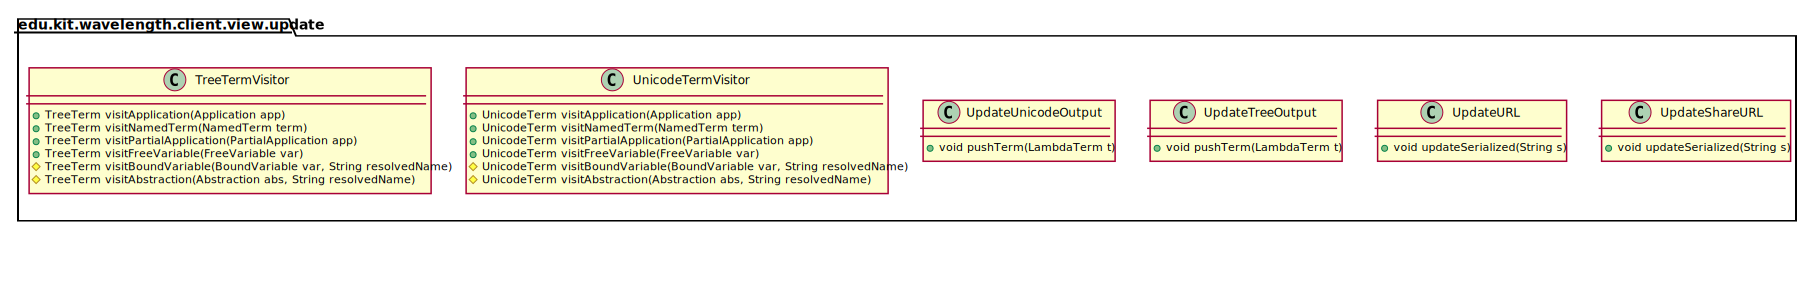
\includegraphics[width=\textwidth]{packageDiagrams/updatePackage}
\end{figure}


\subsubsection{Class \texttt{UpdateURL}}
\label{type:edu.kit.wavelength.client.view.update.UpdateURL}
Implements: \texttt{\hyperref[type:edu.kit.wavelength.client.view.SerializationObserver]{SerializationObserver}}

Observer that updates the browser URL.

\subsubsection{Class \texttt{UpdateUnicodeOutput}}
\label{type:edu.kit.wavelength.client.view.update.UpdateUnicodeOutput}
Implements: \texttt{\hyperref[type:edu.kit.wavelength.client.view.execution.ExecutionObserver]{ExecutionObserver}}

Observer that updates the \texttt{UnicodeOutput} with a new term if it is displayed.

\subsubsection{Class \texttt{UpdateTreeOutput}}
\label{type:edu.kit.wavelength.client.view.update.UpdateTreeOutput}
Implements: \texttt{\hyperref[type:edu.kit.wavelength.client.view.execution.ExecutionObserver]{ExecutionObserver}}

Observer that updates the \texttt{TreeOutput} with a new term if it is displayed.

\subsubsection{Class \texttt{UpdateShareURL}}
\label{type:edu.kit.wavelength.client.view.update.UpdateShareURL}
Implements: \texttt{\hyperref[type:edu.kit.wavelength.client.view.SerializationObserver]{SerializationObserver}}

Observer that updates the URL in the share panel.

\subsubsection{Class \texttt{UnicodeTermVisitor}}
\label{type:edu.kit.wavelength.client.view.update.UnicodeTermVisitor}
Extends: \texttt{\hyperref[type:edu.kit.wavelength.client.model.term.ResolvedNamesVisitor]{ResolvedNamesVisitor}}

Visitor for generating the output of a \texttt{LambdaTerm} for the \texttt{UnicodeOutput} view.

\subsubsection{Class \texttt{TreeTermVisitor}}
\label{type:edu.kit.wavelength.client.view.update.TreeTermVisitor}
Extends: \texttt{\hyperref[type:edu.kit.wavelength.client.model.term.ResolvedNamesVisitor]{ResolvedNamesVisitor}}

Visitor for generating the output of a \texttt{LambdaTerm} for the \texttt{TreeOutput} view.

\subsection{Package \lstinline{edu.kit.wavelength.client.view.webui.component}}
\label{pkg:edu.kit.wavelength.client.view.webui.component}
The \texttt{component} package contains different classes that make up the user interface (UI).

Most of the classes implement the adapter pattern and wrap corresponding GWT-UI classes. 
These classes are \texttt{\lnk{Checkbox}}, \texttt{\lnk{LabeledButton}}, \texttt{\lnk{OptionBox}}, 
\texttt{\lnk{PopUpTextBox}}, \texttt{\lnk{TextField}}, \texttt{\lnk{VisualButton}} and \texttt{\lnk{WindowFocus}}.
Adapting the classes not only achieves consistent naming and functionality for the UI components
but also allows for easy mocking of the classes.

Additionally a few classes are specially designed for the Wavelength IDE. The \texttt{\lnk{Editor}} 
class is implemented by the Monaco Editor API which provides a means for advanced editor functionalities. 
\texttt{\lnk{TreeOutput}} and \texttt{\lnk{UnicodeOutput}} are both interactive visualizations of 
\texttt{\hyperref[type:edu.kit.wavelength.client.model.term.LambdaTerm]{LambdaTerm}}s. They display 
the result of a calculation to the user and also allow the user to request precises calculation steps.

By wrapping the GWT-UI classes behind an adapter, all classes in the \texttt{component} package can
be hidden behind a combination of different interfaces from the \texttt{\pkglnk{view.api}}.
%TODO was ist so toll daran, die hinter den Interfaces zu verstecken?

\begin{figure}[H]
	\centering
	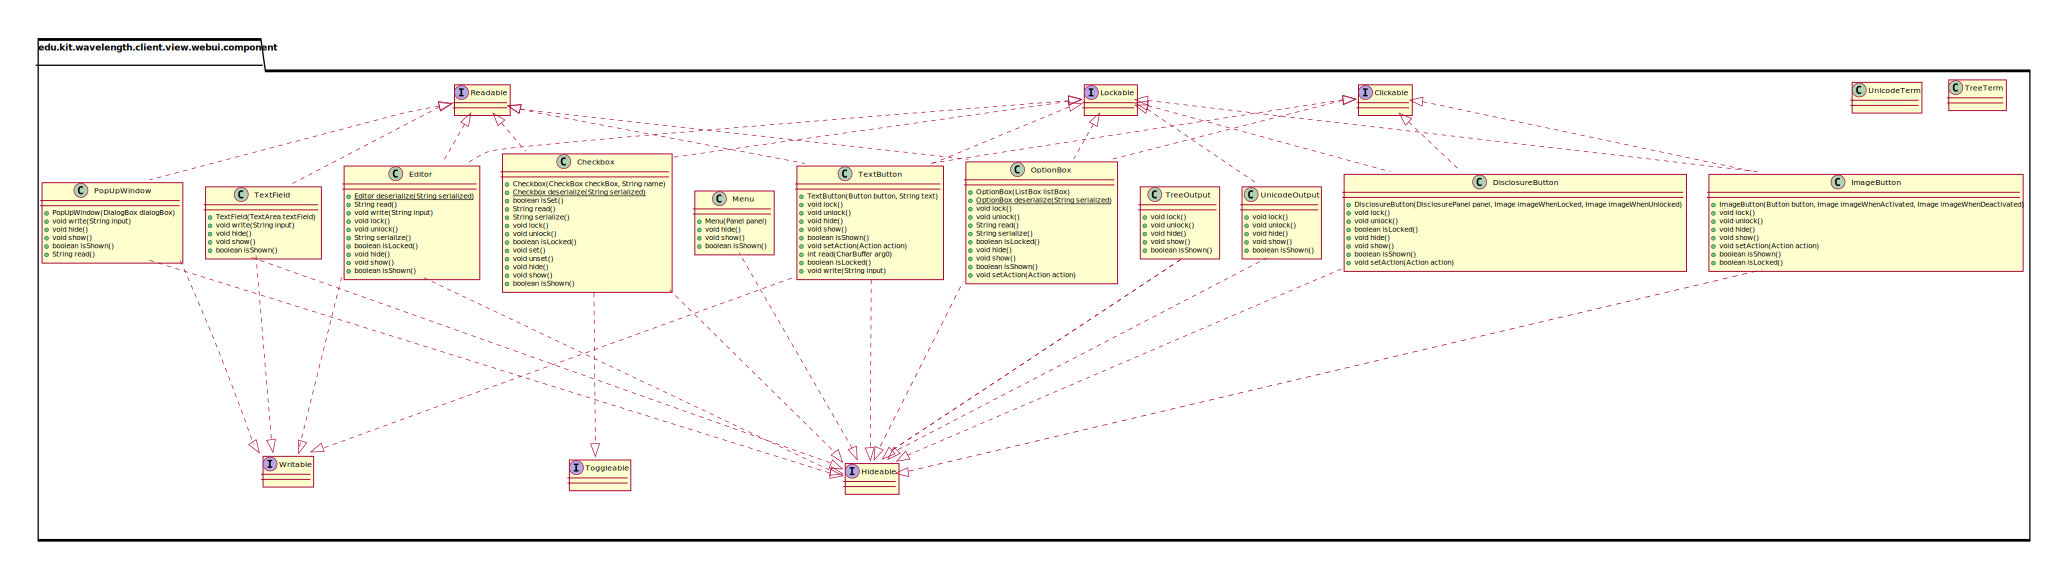
\includegraphics[width=\textwidth]{packageDiagrams/componentsPackage}
\end{figure}


\subsubsection{Class \texttt{UnicodeTerm}}
\label{type:edu.kit.wavelength.client.view.webui.component.UnicodeTerm}
Represents the visual display of a lambda term in text with unicode symbols.

\subsubsection{Class \texttt{UnicodeOutput}}
\label{type:edu.kit.wavelength.client.view.webui.component.UnicodeOutput}
Implements: \texttt{\hyperref[type:edu.kit.wavelength.client.view.api.Lockable]{Lockable}}, \texttt{\hyperref[type:edu.kit.wavelength.client.view.api.Hideable]{Hideable}}

Displays lambda terms in text format with unicode symbols.

\subsubsection{Class \texttt{TreeTerm}}
\label{type:edu.kit.wavelength.client.view.webui.component.TreeTerm}
Represents the visual display of a lambda term as a tree.

\subsubsection{Class \texttt{TreeOutput}}
\label{type:edu.kit.wavelength.client.view.webui.component.TreeOutput}
Implements: \texttt{\hyperref[type:edu.kit.wavelength.client.view.api.Lockable]{Lockable}}, \texttt{\hyperref[type:edu.kit.wavelength.client.view.api.Hideable]{Hideable}}

Displays lambda terms in tree format.

\subsubsection{Class \texttt{TextField}}
\label{type:edu.kit.wavelength.client.view.webui.component.TextField}
Implements: \texttt{\hyperref[type:edu.kit.wavelength.client.view.api.Hideable]{Hideable}}, \texttt{\hyperref[type:edu.kit.wavelength.client.view.api.Writable]{Writable}}, \texttt{\hyperref[type:edu.kit.wavelength.client.view.api.Readable]{Readable}}

A TextField is an adapter class for a GWT TextArea.
 
 A TextField can only be read. It provides a means to display text to the User
 and can be hidden and shown.

Constructors:
\begin{itemize}
\item \texttt{TextField(TextArea textField)}

Constructs a new and empty TextField.

\texttt{textField}: The GWT TextArea that this class wraps.

\end{itemize}

\subsubsection{Class \texttt{TextButton}}
\label{type:edu.kit.wavelength.client.view.webui.component.TextButton}
Implements: \texttt{\hyperref[type:edu.kit.wavelength.client.view.api.Lockable]{Lockable}}, \texttt{\hyperref[type:edu.kit.wavelength.client.view.api.Hideable]{Hideable}}, \texttt{\hyperref[type:edu.kit.wavelength.client.view.api.Writable]{Writable}}, \texttt{Readable}, \texttt{\hyperref[type:edu.kit.wavelength.client.view.api.Clickable]{Clickable}}

A LabeldButton is an adapter class that wraps a GWT Button.

 It is labeled by text and can be blocked and unblocked to prevent the User
 from interacting with it. In Addition its behavior can be changed. This means
 that the name of the label and the action that is performed when clicking
 this button can be changed.

Constructors:
\begin{itemize}
\item \texttt{TextButton(Button button, String text)}

Creates a new LabeledButton.

\texttt{button}: the wrapped \texttt{Button}

\texttt{text}: The label and name of this Button

\end{itemize}

\subsubsection{Class \texttt{PopUpWindow}}
\label{type:edu.kit.wavelength.client.view.webui.component.PopUpWindow}
Implements: \texttt{\hyperref[type:edu.kit.wavelength.client.view.api.Writable]{Writable}}, \texttt{\hyperref[type:edu.kit.wavelength.client.view.api.Hideable]{Hideable}}, \texttt{\hyperref[type:edu.kit.wavelength.client.view.api.Readable]{Readable}}

The PopUpTextBox is an adapter class for the GWT DialogeBox
 
 It is represented by a PopUpWindow that holds a TextField and possibly some
 buttons (e.g. a close Button). It can be hidden or shown. Content can be written and read from the
 TextField.

Constructors:
\begin{itemize}
\item \texttt{PopUpWindow(DialogBox dialogBox)}

Creates a new and empty PopUpTextBox.

\texttt{dialogBox}: the wrapped \texttt{DialogBox}

\end{itemize}

\subsubsection{Class \texttt{OptionBox}}
\label{type:edu.kit.wavelength.client.view.webui.component.OptionBox}
Implements: \texttt{\hyperref[type:edu.kit.wavelength.client.view.api.Clickable]{Clickable}}, \texttt{\hyperref[type:edu.kit.wavelength.client.view.api.Hideable]{Hideable}}, \texttt{\hyperref[type:edu.kit.wavelength.client.view.api.Lockable]{Lockable}}, \texttt{\hyperref[type:edu.kit.wavelength.client.view.api.Readable]{Readable}}, \texttt{\hyperref[type:edu.kit.wavelength.client.model.serialization.Serializable]{Serializable}}

A OptionBox is an adapter class for a GWT ListBox.
 
 It provides a means for the User to set Options for a calculation. This Box
 can be blocked and unblocked if changing the Options must not be possible.

Constructors:
\begin{itemize}
\item \texttt{OptionBox(ListBox listBox)}

Constructs a new and empty OptionBox.

\texttt{listBox}: the wrapped \texttt{ListBox}

\end{itemize}

Static methods:
\begin{itemize}
\item \texttt{\hyperref[type:edu.kit.wavelength.client.view.webui.component.OptionBox]{OptionBox} deserialize(String serialized)}

Creates a new OptionBox from the specified serialized string.

\texttt{serialized}: serialized string, as created in serialize

Returns: new OptionBox

\end{itemize}

\subsubsection{Class \texttt{Menu}}
\label{type:edu.kit.wavelength.client.view.webui.component.Menu}
Implements: \texttt{\hyperref[type:edu.kit.wavelength.client.view.api.Hideable]{Hideable}}

This class wraps GWT's \texttt{Panel} and represents a menu.

Constructors:
\begin{itemize}
\item \texttt{Menu(Panel panel)}

Creates a new Menu.

\texttt{panel}: the wrapped \texttt{Panel}

\end{itemize}

\subsubsection{Class \texttt{ImageButton}}
\label{type:edu.kit.wavelength.client.view.webui.component.ImageButton}
Implements: \texttt{\hyperref[type:edu.kit.wavelength.client.view.api.Lockable]{Lockable}}, \texttt{\hyperref[type:edu.kit.wavelength.client.view.api.Hideable]{Hideable}}, \texttt{\hyperref[type:edu.kit.wavelength.client.view.api.Clickable]{Clickable}}

An ImageButton is an adapter class that wraps a GWT Button.

 It is represented by an \texttt{Image}. The representing image changes if the
 Button is deactivated or not. In addition it can be hidden from the UI.

Constructors:
\begin{itemize}
\item \texttt{ImageButton(Button button, Image imageWhenActivated, Image imageWhenDeactivated)}

Creates a new VisualButton.

\texttt{button}: the wrapped \texttt{Button}

\texttt{imageWhenActivated}: The image that is shown when the Button is active.

\texttt{imageWhenDeactivated}: The image that is shown when the Button is deactivated.

\end{itemize}

\subsubsection{Class \texttt{Editor}}
\label{type:edu.kit.wavelength.client.view.webui.component.Editor}
Implements: \texttt{\hyperref[type:edu.kit.wavelength.client.view.api.Readable]{Readable}}, \texttt{\hyperref[type:edu.kit.wavelength.client.view.api.Writable]{Writable}}, \texttt{\hyperref[type:edu.kit.wavelength.client.view.api.Hideable]{Hideable}}, \texttt{\hyperref[type:edu.kit.wavelength.client.view.api.Lockable]{Lockable}}, \texttt{\hyperref[type:edu.kit.wavelength.client.model.serialization.Serializable]{Serializable}}

This Editor is the main means for the user to input content into the
 application.
 
 The User can input the Terms he wants to calculate. In Addition text can be
 written into the Editor to communicate with the User. The Editor can be
 blocked too to prevent the User from changing its content.

Static methods:
\begin{itemize}
\item \texttt{\hyperref[type:edu.kit.wavelength.client.view.webui.component.Editor]{Editor} deserialize(String serialized)}

Creates a new Editor from the specified serialized string.

\texttt{serialized}: serialized string, as created in serialize

Returns: new Editor

\end{itemize}

\subsubsection{Class \texttt{DisclosureButton}}
\label{type:edu.kit.wavelength.client.view.webui.component.DisclosureButton}
Implements: \texttt{\hyperref[type:edu.kit.wavelength.client.view.api.Clickable]{Clickable}}, \texttt{\hyperref[type:edu.kit.wavelength.client.view.api.Hideable]{Hideable}}, \texttt{\hyperref[type:edu.kit.wavelength.client.view.api.Lockable]{Lockable}}

Button that slides open a panel when clicked.

Constructors:
\begin{itemize}
\item \texttt{DisclosureButton(DisclosurePanel panel, Image imageWhenLocked, Image imageWhenUnlocked)}



\texttt{panel}: Panel to adapt (this is the "Button" with the sliding mechanism itself - not the panel within it)

\texttt{imageWhenLocked}: Image to display when button is locked

\texttt{imageWhenUnlocked}: Image to display when button is unlocked

\end{itemize}

\subsubsection{Class \texttt{Checkbox}}
\label{type:edu.kit.wavelength.client.view.webui.component.Checkbox}
Implements: \texttt{\hyperref[type:edu.kit.wavelength.client.view.api.Readable]{Readable}}, \texttt{\hyperref[type:edu.kit.wavelength.client.view.api.Hideable]{Hideable}}, \texttt{\hyperref[type:edu.kit.wavelength.client.view.api.Toggleable]{Toggleable}}, \texttt{\hyperref[type:edu.kit.wavelength.client.model.serialization.Serializable]{Serializable}}, \texttt{\hyperref[type:edu.kit.wavelength.client.view.api.Lockable]{Lockable}}

This class wraps GWT's \texttt{CheckBox}.

Constructors:
\begin{itemize}
\item \texttt{Checkbox(CheckBox checkBox, String name)}

Creates a new Checkbox

\texttt{checkBox}: the wrapped \texttt{CheckBox}

\texttt{name}: the text shown next to the checkbox

\end{itemize}

Static methods:
\begin{itemize}
\item \texttt{\hyperref[type:edu.kit.wavelength.client.view.webui.component.Checkbox]{Checkbox} deserialize(String serialized)}

Creates a new Checkbox from the specified serialized string.

\texttt{serialized}: serialized string, as created in serialize

Returns: new Checkbox

\end{itemize}

\subsection{Package \lstinline{edu.kit.wavelength.client}}
\label{pkg:edu.kit.wavelength.client}
Overview of \texttt{edu.kit.wavelength.client} with UML diagram.


\subsubsection{Class \texttt{Wavelength}}
\label{type:edu.kit.wavelength.client.Wavelength}
This class marks the entry point of the application.

Methods:
\begin{itemize}
\item \texttt{void onModuleLoad()}

This method is called when the application is first started. It initializes
 the application's \texttt{App} class.

\end{itemize}

